% !TEX root = mythesis.tex

%==============================================================================
\chapter{Neutrino Analysis $60^\circ < \theta < 75^\circ$}
\label{sec:DGL}
%==============================================================================
This chapter gives a brief summary of the neutrino search performed for the zenith range $60^\circ < \theta < 75^\circ$. The neutrino search is separated in different angular range to maximise the performance of the detector array in this case the SD for the search. The chapter aims to cover the expected signature in terms of measurable quantities in the Pierre Auger Observatory for the particular angular range, the neutrino simulation used to develop the analysis, the reconstruction chain used along with the quality cuts used for such an analysis. Further, the quality cuts are analysed in more detail especially in the context of improving the capability of the search by the usage of MoPS and ToTd. In the end the improvements to both the diffused and point source neutrino searches with the new triggers are quantified.


\section{SD Neutrino signature $60^{\circ} < \theta < 75^{\circ}$}
\label{sec:sig_DGL}

The strategy and method to detect neutrino showers in this angular range with the SD remains the same as mentioned before i.e to try detecting showers that develop late and have more electromagnetic or "young" shower front at ground. In terms of signal in the SD array the young shower is expected to be spread over a longer time period typically hundreds of nanoseconds and have a lower maximum peak compared to signal induced by older showers which are spread over tens of nanoseconds and have a higher maximum peak. A comparison of the difference between the induced SD signal from a young and old shower arriving from the same zenith angle is presented in fig. ~\ref{}. However, such differences in signals and the ability of the SD to differentiate between a neutrino induced and a proton/ heavy nuclei induced shower disappears for vertical showers($\Theta < 60^{\circ}$). For vertical showers a cosmic ray induced shower does not have enough time to develop because of the limited thickness of the atmosphere. At these zenith angles a high energy CR induced EAS can mimic the expected young shower signature of a neutrino induced EAS at ground. Thus, currently the neutrino searches at the Pierre Auger Observatory are limited to zenith angles above $60^\circ$ where it is much easier to separate a neutrino induced EAS from a CR induced EAS. Since we are also searching for young showers which have not fully developed till they are detected at ground, reconstructed energy cannot be used as a discrimination criterion.      

To select the longer signals in the SD one of the variables that was used in erstwhile neutrino searches is the fraction of ToT-T2 triggered signals in the recorded event. As mentioned in the previous chapter this trigger is tuned to select broader signals which for an inclined shower is evidence of a young shower. For the search presented in this thesis along with the ToT-T2, the ToTd and MoPS are also used. Both ToTd and MoPS as mentioned in sec.~\ref{} help further increase the selection efficiency for broader signals by reducing the impact of low energy muons. These muons which form the majority of the background at low zenith angles of the selected search range. Thus, these triggers are impactful in increasing the separation power for low energy($\leq$ 1 EeV) neutrino showers. Another important variable which is used to judge the width of the signals is Area Over Peak (AoP). The AoP is defined as the ratio of the integrated signal of the station over the biggest value or peak of the signal. The AoP is calibrated in such a way that narrow/ old shower signals have AoP ~ 1 while broad/old shower signals have AoP $\geqslant $ 1. 



\section{Neutrino Simulations}
\label{sec:sim_DGL}
To characterise the neutrino search ability of the Pierre Auger Observatory Monte Carlo simulations of EASs induced by UHE$\nu$s are required. The simulations were produced in two parts by the Pierre Auger Collaboration Monte Carlo task based on the GAP note ~\ref{}. There are six possible neutrino interaction chanels due to the three possible neutrino flavors with each having two possible channels(CC or NC). However, for simulations these are envisioned to be characterised by just two sets of simulations. For the NC channel since the EAS induced by three neutrino flavors has the exact same signature for our detector only $\nu_e$ NC simulations were performed to estimate the NC contribution of all the three flavors to the final exposure. 

For the CC interactions in the case of $\nu_{\mu}$ the resulting high energy muon has a high probability of evading detection. This is very similar to the NC interaction where the resultant secondary neutrino also carries approximately 80\% of the primary energy. Thus, after taking into account the appropriate crossection, in principle the NC simulations can be used to also estimate the contribution of $\nu_{\mu}$ CC channel.  

In the case of $\nu_{\tau}$ CC interactions where the resulting $\tau$ especially at higher energies($\geq $EeV) can decay and also initiate a secondary shower resulting in a "double bang" like signature in the Observatory. In the context of this thesis such signatures are not accounted for and the $\nu_{\tau}$ CC interaction is treated in the same way as the $\nu_{\mu}$ CC interaction resulting in a possible underestimation of the Observatory to $\nu_{\tau}$ events. A future $\nu_{\tau}$ simulation library is currently being prepared by the Pierre Auger Collaboration Monte Carlo task and could help extend this analysis in the future.

Thus, in summary $\nu_e$ CC and NC simulations can be considered to be good approximations to estimate the contributions of all the other channels to the overall exposure of the Observatory.

\subsection{Atmospheric Shower simulations}
\label{subsec:sim_EAS}
The first part included using CORSIKA~\ref{} to generate the EAS initiated by a $\nu$ primary. This involves simulating the primary neutrino-nucleon interaction which is performed in CORSIKA using the HERWIG code. Further options such as CHARM to track charm secondaries are not used. Also since only $\nu_e$ simulations are simulated, the TAULEP option which handles $\nu_{\tau}$ and $\overline{\nu_{\tau}}$ is also not used. The systematic uncertainties related to the primary interaction estimator is discussed later in section~\ref{}. CORSIKA further tracks the primary interaction products as they travel in the atmosphere towards the ground constituting the air shower. CORSIKA offers a wide variety of choice regarding selecting the hadronic interaction model. For the simulations used in this study separate high and low energy hadronic interaction models were used. For energies higher than 200 GeV three high energy hadronic models QGSJETT~\cite{}, SYBILL~\cite{} and EPOS-LHC~\cite{} were compared. The results of the comparison are mentioned in detail in Appendix~\ref{}. Since the differences between the models are not that significant for the neutrino analysis ....dash..... was chosen as the high energy interaction model. For lower energies FLUKA~\cite{} was chosen. The systematic uncertainities arising from different models are discussed in section~\ref{}.  

To account for the curvature of the Earth which is especially important for the zenith angles studied, the EGS4~\ref{} Monte-Carlo method is chosen to simulate the electromagnetic component of the shower. The analytical NKG~\ref{} method which is also available but is not used for these simulations since it vastly underestimates the maximum of the electromagnetic component due to the fact it does not account for a curved atmosphere.    




Both CC and NC showers were simulated for fixed energy steps of log(E/eV) = 0.5 in the range $10^{17}-10^{20.5}$eV. The number of simulated showers was varied depending on the Energy, atmospheric depth of interaction and the injected zenith angle. More showers were simulated at lower energies and the energy dependent numbers are tabulated in table~\ref{}. Further, for both the interaction channels within the zenith angle range $60^{\circ}-70^{\circ}$ the neutrinos were forced to interact at fixed atmospheric depths in steps of 100 g cm$^{-2}$. The injection points both close to the ground where a neutrino shower might have a lower trigger efficiency and close to the top of the atmosphere where a neutrino induced shower might mimic one induced by a proton are rejected for the simulations. The azimuthal angle is left free and can take any value between 0$^{\circ}$ and 360$^{\circ}$. The simulated depths for each zenith angle bin are summarised in table~\ref{}. 

For each (E,$\theta_{MC}$,X) bin the primary shower 













\begin{figure}[t!]
\centering
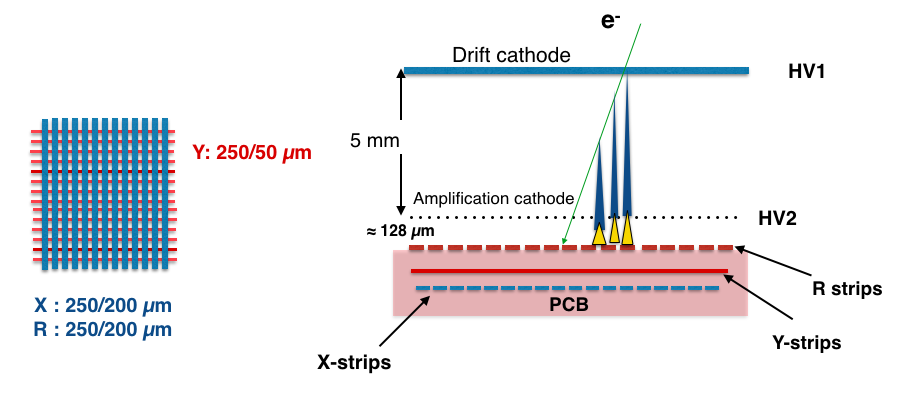
\includegraphics[width=\textwidth]{thesis_figures/NA64_MM.png}
\caption{Left: Strip dimensions of the modules, Right:NA64 Micromega's working principle~\cite{Banerjee:2017mdu}}
\label{fig:Micromegas_na64}
\end{figure}

\subsection{Gas Electron Multiplier}
\label{sec:GEM}

 \begin{figure}[t!]
 \centering
   \begin{minipage}[t]{.45\textwidth}
     \centering
     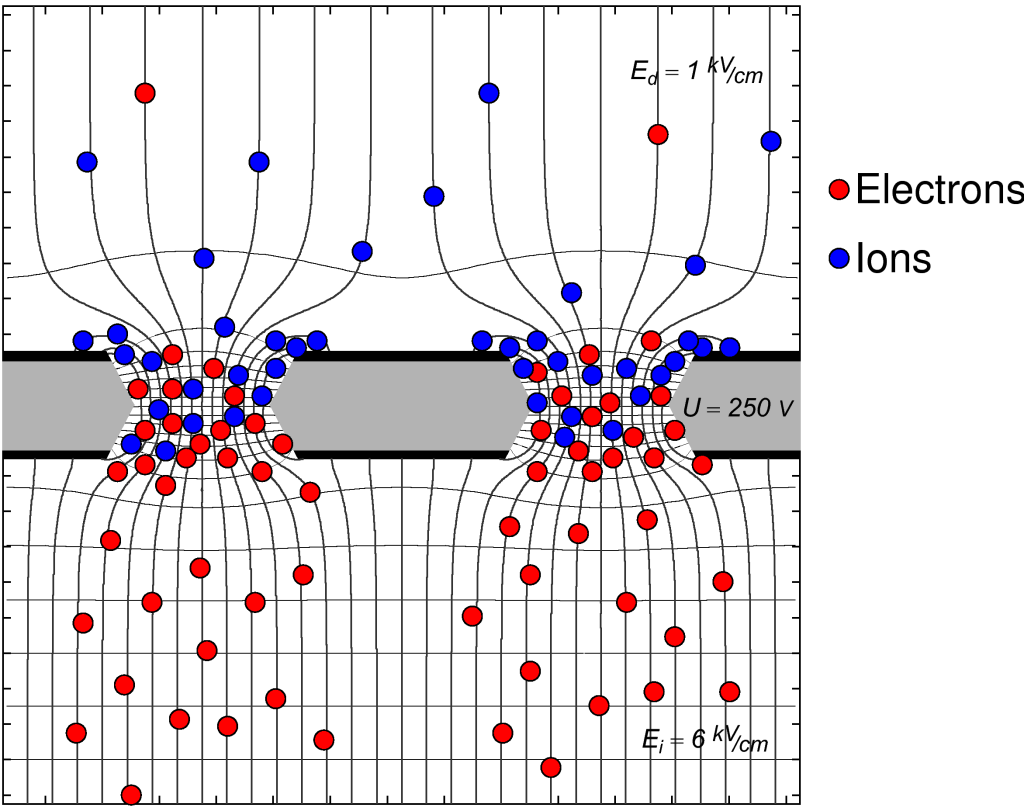
\includegraphics[width=\linewidth]{thesis_figures/GEM_field.png}

     \caption{A sketch of GEM field lines~\cite{GEM_field}.}
     \label{fig:GEM_field}
   \end{minipage}
   \hfill
   \begin{minipage}[t]{.45\textwidth}
     \centering
     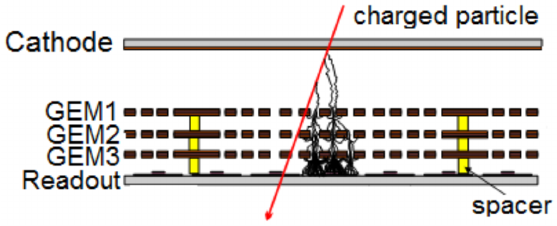
\includegraphics[width=\linewidth]{thesis_figures/GEM_process.png}
     \caption{Schematic of a triple GEM detector along with the working principle~\cite{article_GEM_pic}}
     \label{fig:Triple_GEM}
   \end{minipage}
 \end{figure}

\section{Track-Reconstruction Algorithm}

\subsection{Linear Regression}
\label{sec:Linear_Regression}
Linear regression for track fitting involves fitting a straight line to the data points, hits in our case with the condition that the total error is minimized. The total uncertainty is calculated as a sum of squares of individual measurement errors. Since the final result is dependent on minimizing the sum of the squares this approach to linear regression is known as least-squares approach. A simple mathematical description of the method is given below.

The equation of a straight line is given by $y=mx + c$, where $m$ is the slope of the line and $c$ is the intercept on the $y$ axis in a Cartesian coordinate system. The final goal is to obtain a good estimate for the two parameters $m$ and $c$. To obtain this estimate the square of error needs to be minimized. The error is the difference between the actual measurement $(x_i,y_i)$ and the prediction from our model, the equation of straight line. This error is also known as the residual and is defined as $r_i = y_i - m x_i - c $ for an $i^{th}$ measurement. Suppose that $n$ hits are measured then to obtain an estimate for $m$ and $c$ we need to minimize $\sum_{i=1}^n r_i^2$. The minimized estimates have the following values:
\begin{equation}
      \text{min}(m) = \frac{\sum_{i=1}^n x_i y-i - 1/n \sum_{i=1}^n x_i \sum_{i=1}^n y-i}{\sum_{i=1}^n x_i^2 - 1/n ()\sum_{i=1}^n x_i)^2}  = \frac{\bar{xy} - \bar{x}\bar{y}}{\bar{x^2-\bar{x}^2}}
\end{equation}
\begin{equation}
      \text{min}(c) = \bar{y} - \text{min}(m) \bar{x}
\end{equation}

A more detailed mathematical description can be found in \cite{Linear_regression}. The quality of the fit can be evaluated by calculating the reduced chi-square $\chi^2_{red}=\frac{\chi^2}{ndf.}=\frac{1}{ndf.}\sum_i \frac{(r_i)^2}{\sigma^2}$ where $\sigma$ is the resolution of each detector which might not be equal and ndf. are the number of degrees of freedom available for the fit.

Linear regression can also be used for NA64 to fit for the bending due to the magnets by replacing the model function from the equation of the straight line to some polynomial function. Such a method is called polynomial regression~\cite{STIGLER1974431}.

\begin{figure}[t!]
\centering
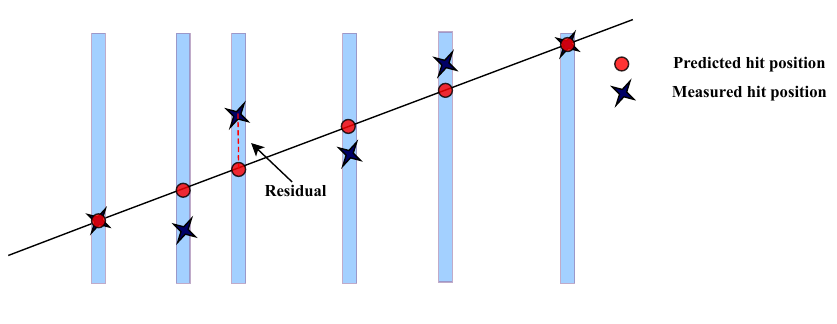
\includegraphics[width=\textwidth]{thesis_figures/linear_reg_new.png}
\caption{Linear regression pictorially. }
\label{fig:linear_regression}
\end{figure}

\subsection{Kalman Filter}
Kalman filter is an estimation technique originally developed to predict rocket trajectories. In particle-physics it is often used as an iterative least-square estimation procedure for track fitting. Following is a brief description of the algorithm for track fitting which closely follows~\cite{Fruhwirth:1987fm,Astier:412374}.

Let's assume for a given track model $x_k$ be the value of the "ideal measurement" at the intersection point between the track and the detector at some point k. This is also called the state vector of the system and in an iterative procedure where the value at location $k$ is obtained from a previous location $k-1$ can be written as :
\begin{equation}
  x_k = f_k(x_{k-1}) + w_k
\end{equation}
where \textbf{f} is the track model propagator function and in this form propogates from detector $k-1$ to $k$ and $w_k$ is a random vector representing the noise between the two detector positions such as multiple scattering perhaps.

\begin{figure}[t!]
\centering
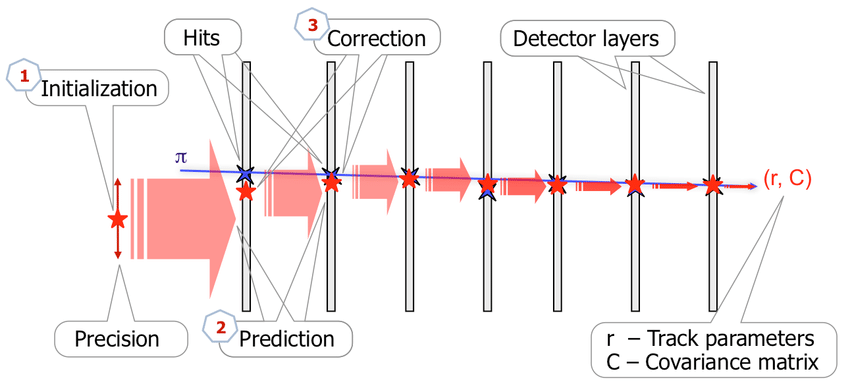
\includegraphics[width=\textwidth]{thesis_figures/KALMAN.png}
\caption{Pictorial representation of the working principle of a Kalman filter ~\cite{article_KALMAN}.}
\label{fig:Kalman_filter}
\end{figure}

Now, the state vector is not a quantity that is measured directly by the detector. If we assume that $m_k$ is the value of the measurement by detector k then it can be given as :
\begin{equation}
  m_k = h_k(x_k) + \epsilon_k
\end{equation}
$h_k(x_k)$ is the function of the state vector measured at the detector which in our case will be a position measurement by our tracking detector. $\epsilon_k$ represents a measurement noise which for an ideal measurement will be zero. We assume that both $w_k$ and $\epsilon_k$ are independent random variables and have a mean value of zero.
For a linearized system,
\begin{equation}
  f_k(x_{k-1}) = F_k x_{k-1}
\end{equation}
\begin{equation}
  h_k(x_{k-1}) = H_k x_k
\end{equation}
There are three key operations that need to be performed for the Kalman filter procedure. These are ordered and described with respect to time specifically to handle multiple scattering in a proper manner.
\begin{description}
  \item $\bullet$~\textbf{Filtering} is estimating the "present" state vector taking into account all the present and "past" measurements. Filtering from $m_1$ to $m_k$ includes filtering $m_1$ to $m_{k-1}$, then propagating from $m_{k-1}$ to $m_k$ and including $m_k$.
  \item $\bullet$~\textbf{Prediction} is estimating the state vector at a "future" time.
  \item $\bullet$~\textbf{Smoothing} is estimating the state vector at any point based on all the measurements.
\end{description}

The basic process can be described as follows. If we have an estimate at position $x_{k-1}$ then it can be extrapolated to position $x_k$ by using the system equation. The estimate at $x_k$ is calculated as a weighted mean between the prediction from the system equation and the measurement from the measurement equation $m_k$. This estimate is passed to all the previous estimates in parallel by using the smoother which is running in a backward direction. Also if there is no process noise $w_k$ then smoothing is equivalent to back extrapolation.

\textbf{System equation:}
\begin{equation}
  x_k = F_k x_{k-1} + w_{k}
\end{equation}
\begin{equation}
  E{w_k} = 0,  \mathrm{Cov[w_k]} = Q_k (1\leq k \leq N)
\end{equation}
\textbf{Measurement Equation:}
\begin{equation}
  m_k = H_k x_{k} + \epsilon_{k}
\end{equation}
\begin{equation}
  E{\epsilon_k} = 0,  \mathrm{Cov[\epsilon_k]} = V_k = G_k^{-1} (1\leq k \leq N)
\end{equation}

As an example here are the different processes for one update step:

\begin{description}
\item $-$ Prediction - Extrapolation of the state vector
      \begin{equation}
        x_k^{k-1} = F_k x_{k-1}
      \end{equation}
      Extrapolation of covariance matrix :
      \begin{equation}
        C_k^{k-1} = F_k C_{k-1} F_k^T + Q_k
      \end{equation}

\item $-$ Filtering - Update of state vector
       \begin{equation}
         x_k = C_k [ \, (C^{k-1}_k)^{-1} x_k^{k-1} + H_k^T G_k m_k ] \,
       \end{equation}
       Update of covariance matrix :
       \begin{equation}
         C_k = [ \, (C^{k-1}_k)^{-1} + H_k^T G_k H_k ]^{-1} \,
       \end{equation}

\item $-$ Smoothing - Smoothed state vector
      \begin{equation}
        x_k^{N} = x_k + A_k(x_{k+1}^N - x_{k+1}^k)
      \end{equation}
      where $A_k$ is called the smoother gain matrix given by: $A_k = C_k F_{k+1} ^T (C_{k+1}^k)^{-1}$

\end{description}
Other information such as residuals $r_k$, covariance matrix of residuals $R_k$ and $\chi^2$ for each step are also calculated and incorporated during the fitting process. A global $\chi^2_{trk}$ is a sum of all chi-squares from filtering. After the Kalman fitting we have three fits for the parameters at a particular hit at position $k$: a track fit for the part upstream i.e  using measurements from 1 till $k$, a backward track fit for the part downstream using measurements from $N$ till $k$ and a fit for the whole track.

The Kalman filter can also be applied for a non-linear system such as in the presence of a magnetic field, by the replacement of the track propagator $f_k$ with the first two terms of of its Taylor series expansion. With this change the procedure is known as extended Kalman filter. This procedure is implemented in the track fitting libraries in CORAL. The computational time of the filter is directly proportional to the number of detector and does not depend much on the total amount of hits in an individual detector. A potential drawback of the algorithm is that it needs initial starting parameters for the state vector and its covariance matrix. This is usually solved by either fitting a small number of measurements with linear regression and then feeding it to the algorithm or by starting with an arbitrary value for the state vector and covariance matrix.

\section{CORAL and PHAST}
CORAL is the reconstruction and analysis software used at COmmon Muon and Proton Apparatus for Structure and Spectroscopy (COMPASS). PHysics Analysis Software Tool (PHAST) was developed later to separate the analysis from reconstruction and works on the output obtained from CORAL. CORAL was envisioned as a modular program that consists of standard libraries for different processes such as track reconstruction and alignment, that are controlled using external option files. Different detectors can be added externally in a detectors table (detectors.dat) which is fed to CORAL along with the measured data file. The libraries of the detectors that are used at the NA64 experiment such as the Micromegas, which are a little different compared to the standard COMPASS ones, were also added to CORAL~\cite{hosgen:2017}.

The track reconstruction process in CORAL works in the following way. The detectors are divided into separate zones either depending on the magnets or depending on obstruction by a detector such as a calorimeter both of which is true especially in the visible mode for NA64. Zones before and after the magnets are fitted with straight line segments depending on the measurements. The line segments in each zone are then bridged together through the magnets which is sped up with an external Dico file. A Dico file consists of all the possible trajectories pre-calculated, for a particular geometry or setup. The last step in the track reconstruction process is a Kalman filter taking the initial information from the previous two steps and running over the entire track piece, combining the measurements into the final prediction. The momentum is determined according to the integrated magnetic field and the bending angle observed for the fitted track. The option file for track reconstruction for NA64 controls the input and output files for the whole process and also contains information about various noise cuts implemented for the detectors which are described in detail in \cite{hosgen:2017}.



%%% Local Variables:
%%% mode: latex
%%% TeX-master: "mythesis"
%%% End:
